\documentclass[11pt,twoside,a4paper]{article}

\newcommand{\RNum}[1]{\uppercase\expandafter{\romannumeral #1\relax}}
\usepackage{cite}
\usepackage{cases}
\usepackage{amsmath,amssymb,amsfonts}
\usepackage{algorithmic}
\usepackage{graphicx}
\usepackage{textcomp}
\usepackage{xcolor}
\usepackage{booktabs} 
\usepackage[ruled]{algorithm2e} 
\def\BibTeX{{\rm B\kern-.05em{\sc i\kern-.025em b}\kern-.08em
    T\kern-.1667em\lower.7ex\hbox{E}\kern-.125emX}}

	\title{\textbf{Fast Privacy Preserved Deep Learning}}
	\author{\sffamily author1$^1$, \sffamily author2$^2$, \sffamily author3$^3$}
	\date{(Dated: \today)}

\begin{document}
\maketitle

\begin{abstract}

\end{abstract}
\section{Introduction}
Lung sick pateients in hospital want to take CT image of chest to detect if their lungs are sick and know the type of disease.
Hospital doesn't have the ability to identify accurately. 
So it needs to ask a technology company who has relative deep learning model for help.
But patients don't want any party except the hospital to get his chest CT images.
At the same time, the technology company also don't want to let its own models leaked to any party.
fast privacy preserved deep learning provides a deep learning prediction method to protect both model data of technology company and privacy data of patients.

\section{Preliminaries}

\subsection{Semi-honest participants}

Participants joining in the whole process will follow rules of agreements. 
They won't deliberately send wrong information.
However, they are curious about another participants' input data.

\subsection{Notations}

We denote a shared variable $x$ by $\langle x\rangle $. 
The secret share of $\langle x\rangle $ held by the $i-th$ party is denoted as $\langle x\rangle ^{i}$, $i\in \{0,1\}$. 
We use additive sharing method through whole paper. Specifically, $x=\langle x\rangle ^{0}+\langle x\rangle ^{1}$.

In our paper, there are two parties to participate in calculation. 
We denote them by $P_{0}$ and $P_{1}$. We use $P_{i}$ to refer to the two parties respectively.

If a variable $x<0$, we set the sign of $x=-1$, else if $x>0$, we set the sign of $x=1$, else if $x=0$, we set the sign of $x=0$.

\section{Comparison between two secret variables}
In this section, we detail the tricks used in the following sections. 
In general, we introduce comparison between a shared secret variable and zero(\textbf{3.2}) 
and comparison between two shared secret variables(\textbf{3.3}).

\subsection{multiplication of two shared variables}

$P_{i}$ holds $\langle x\rangle ^{i}$ and $\langle y\rangle ^{i}$.
$P_{i}$ wants to have $\langle z\rangle ^{i}$, 
s.t. $\langle z\rangle ^{0}+\langle z\rangle ^{1}=(\langle x\rangle ^{0}+\langle x\rangle ^{1})
\cdot (\langle y\rangle ^{0}+\langle y\rangle ^{1})$

This multiplication relys on Beaver’s multiplication triples $(a,b,c)$, where $c=a \cdot b$. 
The multiplication triples can be distributed by trsted setup. 
The trusted setup sends secret shares $\langle a\rangle ^{i},\langle b\rangle ^{i},\langle c\rangle {i}$.

$P_{i}$ computes $\langle e\rangle ^{i}=\langle x\rangle ^{i}-\langle a\rangle ^{i}$ and $\langle f\rangle ^{i}=\langle y\rangle ^{i}-\langle b\rangle ^{i}$.
$P_{i}$ shares $\langle e\rangle^{i}$ and $\langle f\rangle^{i}$ with each other. Then, $P_{i}$ compute the value of $e$ and $f$.

$P_{i}$ sets $\langle z\rangle^{i}=i\cdot e \cdot f + f\cdot \langle a\rangle^{i}+e \cdot \langle b\rangle^{i} + \langle c\rangle^{i}$.

\subsection{Comparison between a shared secret variable and zero}

In convolution neural network, ReLU function is used many times as an activation function. ReLU function needs to campare the input variable and 0.

$$ReLU(x)=\begin{cases}
	x & \text{ if } x > 0 \\ 
	0 & \text{ if } x \leqslant 0  
	\end{cases}$$

Here we design a protocol to compute the sign of shared variable $x$ secretly.

In this paper we introduce the comparison  $(u,p,q)$. s.t. $u=\langle u\rangle ^{0}+\langle u\rangle ^{1}=p\cdot q$.

The general idea of this section is multiply $ x $ by a random number $ u $ to blind the value of $x$. So that $x \cdot u = x \cdot p\cdot q$
Via \textbf{3.1}, $P_{i}$ gets $\langle z\rangle ^{i}$, where $z= u\cdot x$.
Then $P_{0}$ shares the sign of $1/p$ and $P_{1}$ shares the sign of $z/q$.
Since $x  = \frac{x \cdot u}{p\cdot q}=\frac{z}{p\cdot q}$, the sign of $x$ can be easily calculated with product of the sign of $1/p$ and $z/q$.

Concretely, The protocol is run as follow. 

\textbf{Distribution of triples}The trusted setup $TTP$ distributes one multiplication triple and one comparison triple to $P_{0}$ and $P_{1}$.
As for comparison triple, $TTP$ randomly generate triple $(u,p,q)$, s.t. $u=\langle u\rangle ^{0}+\langle u\rangle ^{1}=p\cdot q$. 
Then $TTP$ sends $(\langle u\rangle ^{0}, p)$ to $P_{0}$, and $(\langle u\rangle ^{1}, q)$ to $P_{1}$.

\textbf{Blinding the addition}$P_{0}$ and $P_{1}$ run the multiplication protocol to get $\langle z\rangle ^{0}+\langle z\rangle ^{1}=(\langle u\rangle ^{0}+\langle u\rangle ^{1})\cdot(\langle x\rangle ^{0}+\langle x\rangle ^{1})=u\cdot x$. 
$P_{i}$ shares the value of $\langle z\rangle ^{i}$ and computes  $z=\langle z\rangle ^{0}+\langle z\rangle ^{1}=u\cdot x$. 

\textbf{Computing the sign}$P_{0}$ sets $s ^{0}=1/p$ and $P_{1}$ sets $s^{1}=z/q$. 
It can be found now :

%\begin{align}
	 $$s ^{0}\cdot  s ^{1} = \frac{z}{p\cdot q} 
	                     = \frac{x \cdot u}{p\cdot q}
					     = x$$
%  \end{align}

So the sign of $x$ equals to that of $s ^{0} \cdot s ^{1}$.

$P_{i}$ shares the sign of $ s^{0}$ and $ s ^{1}$. Finally, the sign of $x$ is equal to the sign of $ s^{0}$ and $ s^{1}$.


\textbf{Security proof}: Intuitively, after running a protocol completely, any participants shouldn't have any information about 
true value of the shared variable except for information leaked by the protocol result which cannot be avoided. 
Specifically, If the result of the protpcol is $x>0$. 
$P_{0}$ and $P_{1}$ shouldn't have any information about $x$ except for $x>0$.
If that holds, we think that the protocol is secure.  



Since $P_{0}$ and $P_{1}$ are dual. We just discuss $P_{0}$.

Recall what information $P_{0}$ can get from the protocol: 
$P_{0}$ holds value of $(\langle x\rangle ^{0},\langle u\rangle ^{0},p,z,$the sign of $s^{1},$the sign of $x)$.
Moreover, $P_{0}$ knows two equations and two signs of variables.


	\begin{numcases}{}
	\langle u\rangle ^{0}+\langle u\rangle ^{1}=p\cdot q\\ 
	z=(\langle u\rangle ^{0}+\langle u\rangle ^{1})\cdot(\langle x\rangle ^{0}+\langle x\rangle ^{1})\\ 
	\text{sign of }x \\ 
	\text{sign of }z/q
		\end{numcases}


Obviously, from the former two equations, 
there are three unknown variables $(\langle u\rangle ^{1},\langle x\rangle ^{1},q)$. 
The true value of $\langle x\rangle ^{1}$ can't be computed.
With $(3)$, we discuss in different situations.

\textbf{If} $x=0$, since $z=x\cdot u=0$. So $z/q=0$.

\textbf{If} $x>0$, since $P_{0}$ hold $z$, $P_{0}$ can deduce the sign of $u$ based on $(2)$. 
Similarly, $P_{0}$ can deduce the sign of $q$ based on $(1)$. Then $P_{0}$ can easily get the sign of $z/q$.

$P_{0}$ has already known about the sign of $q$ by considering about the equation 1 and the sign of $q$.

\textbf{If} $x<0$, the situations is the same as $x>0$.

In conclusion, With $(1)(2)(3)$, we can deduce $\text{sign of }z/q$.So $(4)$ can be omitted.
$P_{0}$ can't get information about $x$ more than the sign of $x$ based on $(1)(2)(3)$.

Overall, the protocol leaks no information about $x$ except the sign of $x$. 
As for the purpose of this protocol is to calculate the sign of $x$.
We think that this protocol is secure.
	
\subsection{Comparison between two secret variables}
In Max Pooling Layer, the biggest element of near input elements is chosen to construct the feature map in next layer.
This asks us to design a protocol to compare between two secret variables.

$P_{i}$ has $\langle x\rangle ^{i}$ and $\langle y\rangle ^{i}$.
They wonders $x$ and $y$ which one is bigger.

$P_{i}$ computes $\Delta^{i}=\langle x\rangle ^{i}-\langle y\rangle ^{i}$.


\section{Privacy preserved deep learning}
In this section, we will introduce framework and concret implement of our system of privacy preserved deep learning. 

\subsection{Overview}
Our system involves five characters: Hospital-$Hosp$, AI technology company-$Comp$, cloud sever\_0 $P_{0}$, cloud sever\_1-$P_{1}$ and a trusted setup-$TTP$. Tasks of each characters are as follow.

\begin{figure}[htbp]
	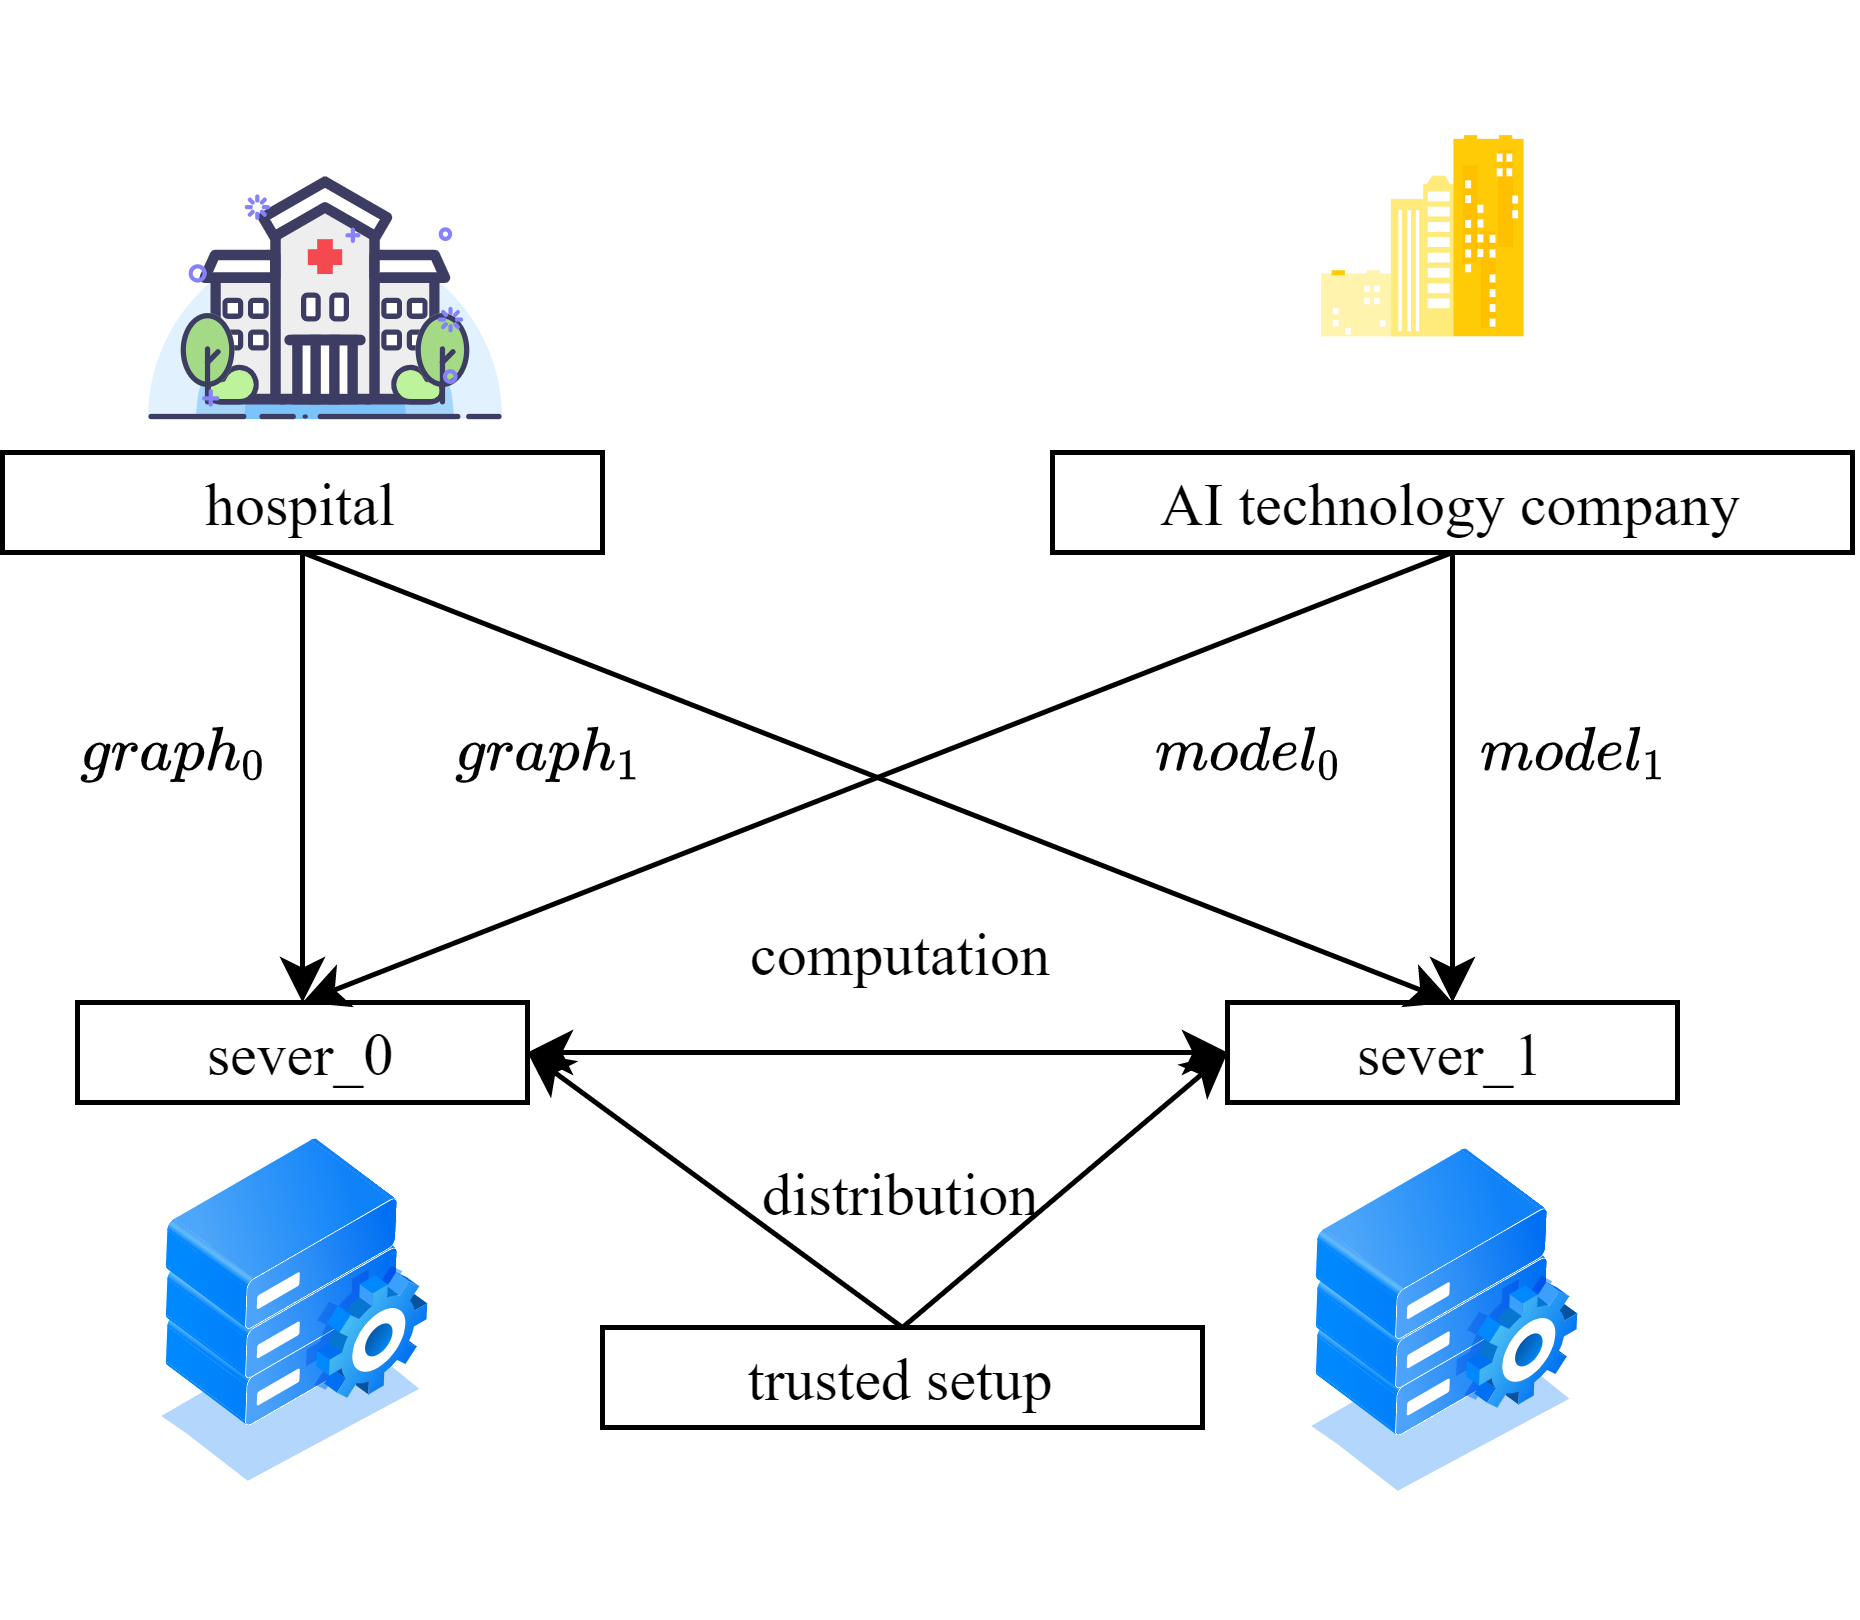
\includegraphics[width=8cm]{framework.png}
	\caption{system framework}
\end{figure}


\textbf{Hospital}-$Hosp$: take CT images of the patient's lungs and distribute two pieces of shared images to two cloud severs.

\textbf{AI technology company}-$Comp$: prepare a trained convolutional neural network model in advance and distribute two pieces of convolution kernel to two cloud severs. 
upon receiving two shared results of Convolutional Layer and Pooling layer from two cloud severs, 
add the shared results to get the real result and conduct the rest part of convolutional neural network.
 
\textbf{Cloud sever\_0}-$P_{0}$ and $P_{1}$: receive images and convolution kernel pieces from $Hosp$ and $Comp$. 
Compute results of Convlutional Layer, Pooling layer and ReLU function on the basis of \textbf{Protocol1-3}.

\textbf{Trusted setup}-$TTP$: distribute Beaver’s multiplication triples and comparison triples. 
This task can be conducted at the very beginning, even long before the protocol running.

\subsection{System Framework}
\textbf{Step1: Distribution}:$\{\}\rightarrow \{P_{i}:(multiplication-triples, comparison-triples, \langle Imag\rangle ^{i}, \langle Conv\rangle ^{i})\}$.
$TTP$ distributes enough Beaver’s multiplication triples and comparison triples to $P_{0}$ and $P_{1}$. 
$Hosp$ distributes two pieces of shared part of CT images $\langle Imag\rangle ^{i}$ to $P_{i}$. 
$Comp$ distributes two pieces of shared part of convolution kernel $\langle Conv\rangle ^{i}$ to $P^{i}$.

\textbf{Step2: Computation of Convolutional Layer}:$\{P_{i}:(multiplication-triples, \langle Imag\rangle ^{i}, \langle Conv_{c}\rangle ^{i})\}\rightarrow \{P_{i}:(\langle Feature_{conv}\rangle ^{i})\}$. 
Based on Protocol1 $P_{0}$ and $P_{1}$ compute Convolutional Layer using the shared data $\langle Imag\rangle $ and $\langle Conv\rangle $. 

\textbf{Step3: Computation of Pooling Layer}. :$\{P_{i}:(comparison-triples, \langle Feature_{conv}\rangle ^{i})\}\rightarrow \{P_{i}:(\langle Feature_{pool}\rangle ^{i})\}$. 
Based on Protocol3 $P_{0}$ and $P_{1}$ compute max Pooling Layer using the shared data $\langle Imag\rangle $ and $\langle Conv\rangle $.

\textbf{Step4: Computation of ReLU function}: $\{P_{i}:(comparison-triples, \langle Feature_{pool}\rangle ^{i})\}\rightarrow \{P_{i}:(\langle Feature_{ReLU}\rangle ^{i})\}$.
Based on Protocol2 $P_{0}$ and $P_{1}$ compute ReLU function using the shared data $\langle Imag\rangle $ and $\langle Conv\rangle $. Generally speaking, a CNN 
model usually has more than 1 Convolutional Layer. If there are more Convolutional Layer to be computed, 
move to \textbf{Step2:} Computation of Convolutional Layer with input:$P_{i}:(multiplication-triples, \langle Feature_{ReLU}\rangle ^{i}, \langle Conv_{c}\rangle ^{i})$

\textbf{Step54: Computation of rest part of CNN}: $\{P_{i}:(\langle Feature_{ReLU}\rangle ^{i})\}\rightarrow \{Comp:(answer)\}$. 
$P_{i}$ sends $(\langle Feature_{ReLU}\rangle ^{i})$ to $Comp$ secretly. $Comp$ continues with the remaining steps via the rest of model 
just like Fully-Connected Layer and Classification Layer.
 
\subsection{Concrete implement}
\textbf{Step1: Distribution}.$TTP$ computes enough Beaver’s multiplication triples $(a,b,c),s.t.c=a\cdot b,$. 
$TTP$ distributes additive secret sharing of Beaver’s multiplication triples to $P_{0}$ and $P_{1}$. 
Specifically, $TTP$ sends $(\langle a\rangle ^{i}, \langle b\rangle ^{i}, \langle c\rangle ^{i})$ to $P_{i}$.
Similarly, $TTP$ prepares enough comparison triples ${u,p,q}, s.t. u=p\cdot q$. 
Then $TTP$ sends $(\langle u\rangle ^{0}, p)$ to $P_{0}$ and $(\langle u\rangle ^{1}, q)$ to $P_{1}$.

Next we introduce the method of sharing matrix. Take $2\times 2$ matrix $A$ for example. 
One who shares the secret of $A$ will randomly chooses $2\times 2$ matrix $R$. 
Elements of  $R\xleftarrow{\$}Z^{*}$.
Then, set $\langle A\rangle ^{0}=R$ and $\langle A\rangle ^{1}=A-R$.
The party sharing the secret sends $\langle A\rangle ^{i}$ to $P_{0}$.

$$A=\begin{bmatrix}
	A_{00}& A_{01} \\ 
	A_{10}& A_{11}
   \end{bmatrix}= \begin{bmatrix}
	R_{00}& R_{01} \\ 
	R_{10}& R_{11}
   \end{bmatrix}+\begin{bmatrix}
   A_{00}- R_{00}& A_{01}-R_{01} \\ 
   A_{10}- R_{10}& A_{11}-R_{11}
   \end{bmatrix}=\langle A\rangle ^{0}+\langle A\rangle ^{1}$$

Following rules mentioned above, $Hosp$ distributes two pieces of shared part of CT images $\langle Imag\rangle ^{i}$ to $P_{i}$. 
$Comp$ distributes two shared part of convolution kernel weight matrix $\langle Conv\rangle ^{i}$ and bias $b^{i}$ to $P_{i}$.

\textbf{Step2: Computation of Convolutional Layer}:$\{P_{i}:(\langle Imag\rangle ^{i}, \langle Conv_{c}\rangle ^{i})\}\rightarrow \{P_{i}:(\langle Feature_{conv}\rangle ^{i})\}$. 
Based on Protocol1 $P_{0}$ and $P_{1}$ using the shared data $\langle Imag\rangle $ and $\langle Conv\rangle $.

Convolution is a frequently-used operation between an matrix (image or feature map) and a convolution kernel.
In this paper, we take one two-dimensional convolution kernel for example. It can be easily generalized to dimensions more than 2 and more convolution kernel.

Let us denote $height\times width$ input image by $A$ , $len\times len$weight matrix of convolution kernel by $B$ and bias by $b$.
$C= conv(A,B)$.
$$C_{k,j}=\sum _{w,l}A_{k+w,j+l}\cdot B_{w,l}+b$$
where $0\leqslant k<height,0\leqslant j<width,0\leqslant w<len,0\leqslant l<len$.

Take notice of the formula, the right side of the multiplication part of equation consisted by multiplication and addition.
Multiplication part can be computed via Protocol1 and the addition part can be operated by adding the secret variable locally. 

We denote $mul_{k+w,j+l}=A_{k+w,j+l}\cdot B_{w,l}$.
$$C_{k,j}=\sum_{w,l} mul_{k+w,j+l}+b$$

To get $C_{k,j}$, $P_{0}$ and $P_{1}$ needs to get $mul_{k+w,j+l}^{0}+mul_{k+w,j+l}^{1}=(A_{k+w,j+l}^{i}+A_{k+w,j+l}^{1-i})\cdot (B_{w,l}^{i}+B_{w,l}^{1-i})$. 

Firstly we focus on how to compute $mul_{k+w,j+l}$. 
When computing multiplication part, there are two situations. 

Situation1: under some circumstance (specifically stated in Step4), 
$P_{i}$ knows that $A_{k+w,j+l}^{0} = A_{k+w,j+l}^{1} = 0$. 
$P_{i}$ set $mul_{k+w,j+l}^{i}=0 $ directly.

Situation2: under general circumstance, $P_{i}$ has $A_{k+w,j+l}^{0}$ and $B_{w,l}^{i}$.

So $P_{0}$ and $P_{1}$ run \textbf{multiplication protocol} to get 
$$mul_{k+w,j+l}^{0}+mul_{k+w,j+l}^{1}=(A_{k+w,j+l}^{0} + A_{k+w,j+l}^{1})\cdot(B_{w,l}^{0}+B_{w,l}^{1})$$
Now, $P_{i}$ holds $mul_{k+w,j+l}^{i}$.

After multiplication part, $P_{i}$ needs to compute $C_{k,j}$ locally.
$$C_{k,j}^{i}=\sum_{w,l} mul_{k+w,j+l}^{i}+b^{i}$$

\textbf{Step3: Computation of Pooling Layer}: $\{P_{i}:(\langle Feature_{conv}\rangle ^{i})\}\rightarrow \{P_{i}:(\langle Feature_{pool}\rangle ^{i})\}$.
Based on Protocol3 $P_{0}$ and $P_{1}$ compute max Pooling Layer using the shared data $\langle Imag\rangle $ and $\langle Conv\rangle $.

\begin{figure}[htbp]
	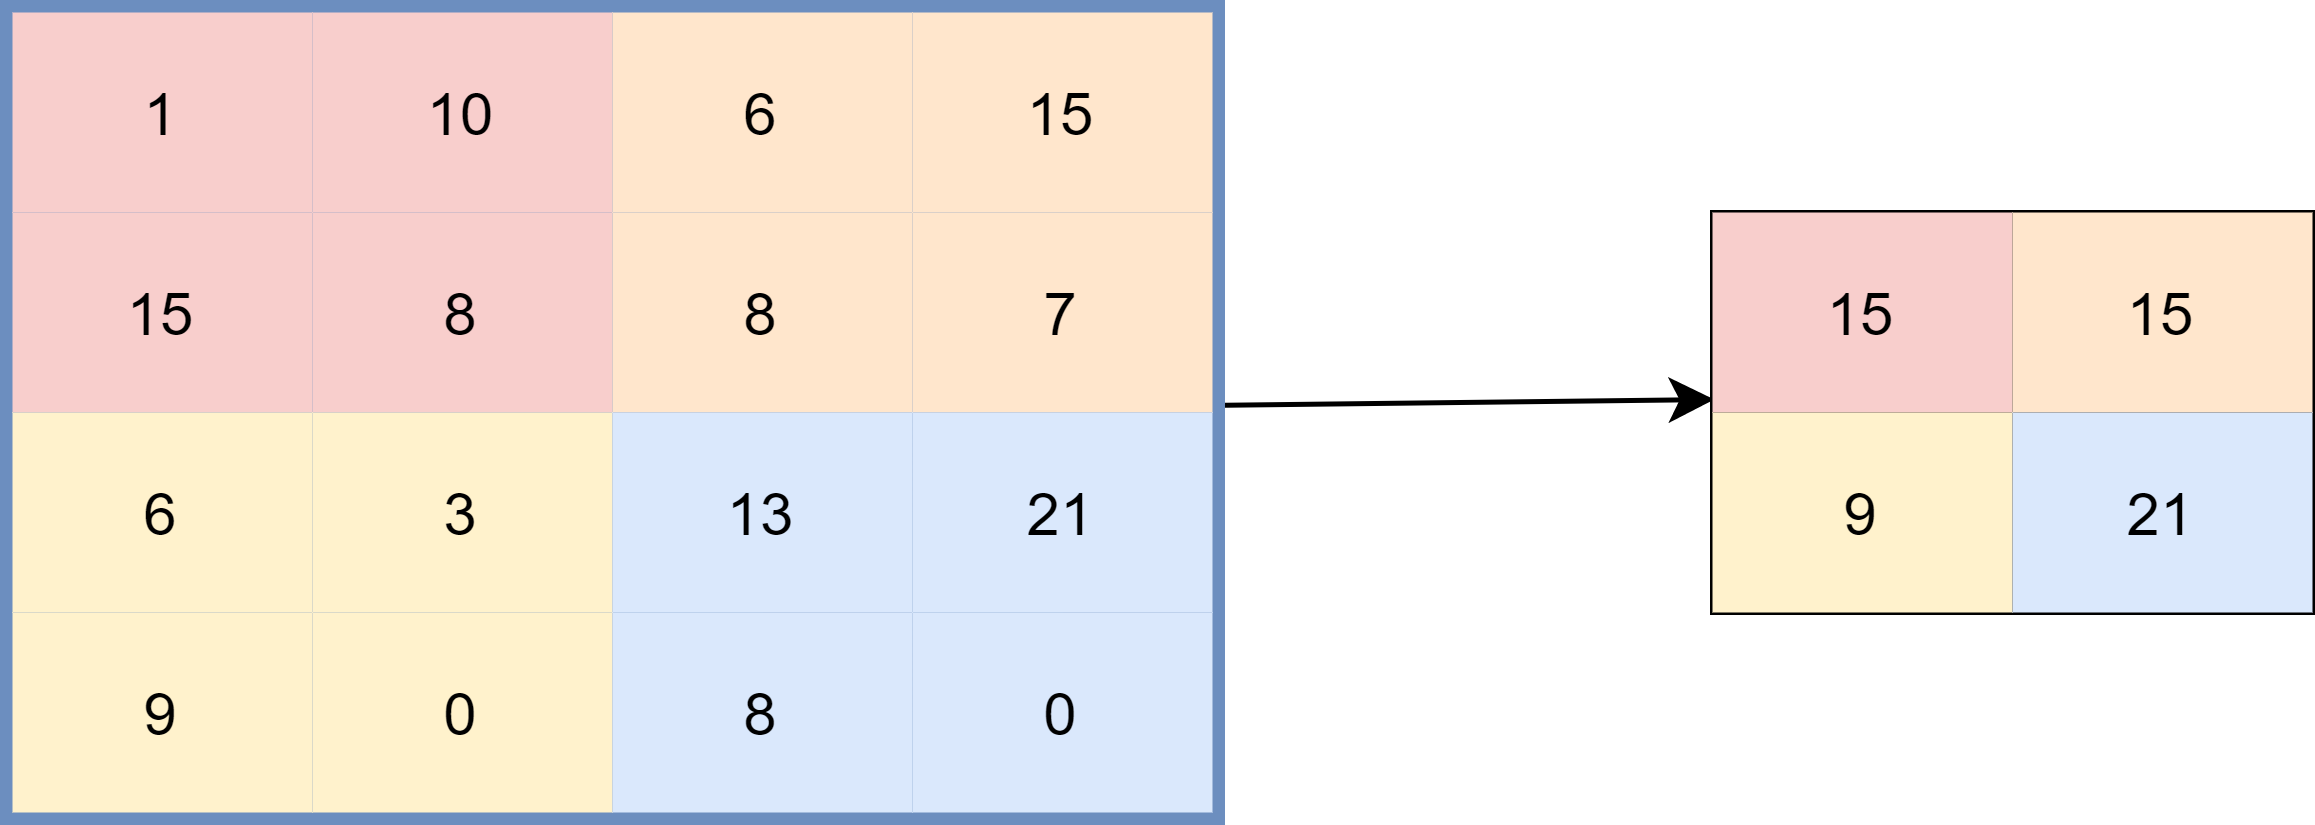
\includegraphics[width=8cm]{pool.png}
	\caption{rules of Pooling Layer}
\end{figure}

In the max Pooling Layer, $P_{0}$ and $P_{1}$ are asked to choose the biggest variable of four near elements to contrust the next feature map.
$P_{0}$ and $P_{1}$ run Protocol3 to compare elements.

By bubble sort, It is easy to see that it takes three times to compute the biggest variable.


\textbf{Step4: Computation of ReLU function}: $\{P_{i}:(\langle Feature_{pool}\rangle ^{i})\}\rightarrow \{P_{i}:(\langle Feature_{ReLU}\rangle ^{i})\}$.
Based on Protocol2 $P_{0}$ and $P_{1}$ compute ReLU function using the shared data $\langle Imag\rangle $ and $\langle Conv\rangle $. 

ReLU function is used in CNN to prevent overfitting. It will set variables which is smaller than 0 to 0 while remain variables bigger than 0.

$$ReLU(x)=\begin{cases}
	x & \text{ if } x > 0 \\ 
	0 & \text{ if } x \leqslant 0  
	\end{cases}$$

$P_{0}$ and $P_{1}$ wonder whether elments of feature map are bigger than 0. They run Protocol2 on input $P_{0}: \langle Feature_{conv}\rangle ^{0},P_{1}:\langle Feature_{conv}\rangle ^{1}$


Generally speaking, a CNN model usually has more than 1 Convolutional Layer. If there are more Convolutional Layer to be computed, 
move to $Step2: Computation of Convolutional Layer$ with input:$P_{i}:(multiplication-triples, \langle Feature_{ReLU}\rangle ^{i}, \langle Conv_{c}\rangle ^{i})$

\textbf{Step5: Computation of rest part of CNN}: $\{P_{i}:(\langle Feature_{ReLU}\rangle ^{i})\}\rightarrow \{Comp:(answer)\}$.$P_{i}:(\langle Feature_{ReLU}\rangle ^{i})$.
$P_{i}$ sends $(\langle Feature_{ReLU}\rangle ^{i})$ to $Comp$ secretly. $Comp$ recovers $Feature_{ReLU}$ by $Feature_{ReLU}=\langle Feature_{ReLU}\rangle ^{0}+\langle Feature_{ReLU}\rangle ^{1}$. 
$Comp$ continues with the the rest of model such as Fully-Connected Layer and Classification Layer.



\section{Conclusion}

\section*{Acknowledgments}
These are acknowledgments. 
\begin{thebibliography}{100}%此处数字为最多可添加的参考文献数量
	\bibitem{article1}This is reference.%title author journal data pages
	\bibitem{book1}This is reference.%title author publish date
\end{thebibliography}

\section{Appendix}

\begin{algorithm}[htbp]
	\caption{Protocol1:multiplication of two shared secret variables}
	\textbf{Input}: $P_{0}$: $\langle x\rangle ^{0}$,$\langle y\rangle ^{0}$\\
	$P_{1}$: $\langle x\rangle ^{1}$,$\langle y\rangle ^{1}$\\
	$TTP$: no\\

	\textbf{Output}: $P_{0}$: $\langle z\rangle ^{0}$\\
	$P_{1}$: $\langle z\rangle ^{1}$\\
	s.t. $\langle z\rangle ^{0}+\langle z\rangle ^{1}=(\langle x\rangle ^{0}+\langle y\rangle ^{0})\cdot(\langle x\rangle ^{1}+\langle y\rangle ^{1}) $\\
\end{algorithm}

\begin{algorithm}[htbp]
	\caption{Protocol2: Comparison between a shared secret variable and zero}
	\textbf{Input}: $P_{0}$: $\langle x\rangle ^{0}$\\
	$P_{1}$: $\langle x\rangle ^{1}$\\
	$TTP$: no\\
	\textbf{Output}:calculate the sign of $x$\\
	~\\
	$TTP$ randomly chooses $\langle u\rangle ^{0}\xleftarrow{\$}Z^{*}, p\xleftarrow{\$}Z^{*}, q\xleftarrow{\$}Z^{*}$\\
	$TTP$ computes $\langle u\rangle ^{1}=p\cdot q-\langle u\rangle ^{0}$\\
	s.t. $\langle u\rangle ^{0}+\langle u\rangle ^{1}=p\cdot q$\\
	$TTP\rightarrow P_{0}$: $(\langle u\rangle ^{0}, p)$\\
	$TTP\rightarrow P_{1}$: $(\langle u\rangle ^{1}, q)$\\
	$P_{0}, P_{1}$ run Protocol1 on input $\{P_{0}:(\langle u\rangle ^{0},\langle x\rangle ^{0}), P_{1}:(\langle u\rangle ^{1},\langle x\rangle ^{1}), TTP()\}$, 
	$P_{0}$ gets $\langle z\rangle ^{0}$ and $P_{1}$ gets $\langle z\rangle ^{1}$, 
	s.t. $\langle z\rangle ^{0}+\langle z\rangle ^{1}=(\langle u\rangle ^{0}+\langle u\rangle ^{1})\cdot(\langle x\rangle ^{0}+\langle x\rangle ^{1})$\\
	$P_{0}\rightarrow P_{1}$: $\langle z\rangle ^{0}$\\
	%$P_{1}\rightarrow P_{0}$: $\langle z\rangle ^{1}$\\
	$P_{1}$ computes $z=\langle z\rangle ^{0}+\langle z\rangle ^{1}$\\

	$P_{0}$ sets $s^{0}=p$\\
	$P_{1}$ sets $s^{1}=z\cdot q$\\
	So that $s^{0}\cdot s^{1}$
	$P_{i}$ sets $sign^{i}=$ the sign of $s^{i}$\\
	$P_{i}$ shares $sign^{i}$ and computes Comparison result $res=sign^{0}\cdot sign^{1}$ \\
	The sign of $x$ equals to $res$\\
\end{algorithm}

\begin{algorithm}[htbp]
	\caption{Protocol3: Comparison between two shared secret variables}
	\textbf{Input}: $P_{0}$: $\langle x\rangle ^{0}$,$\langle y\rangle ^{0}$\\
	$P_{1}$: $\langle x\rangle ^{1}$,$\langle y\rangle ^{1}$\\
	$TTP$: nothing\\
	\textbf{Output}:figure out x and y which one is bigger.\\
	~\\
	$P_{0}$ computes $\Delta^{0}=\langle x\rangle ^{0}-\langle y\rangle ^{0}$\\
	$P_{1}$ computes $\Delta^{1}=\langle x\rangle ^{1}-\langle y\rangle ^{1}$\\
	$P_{0}, P_{1}$ run Protocol2 on input $\{P_{0}:(\Delta^{0}), P_{1}:(\Delta^{1}), TTP()\}$, $P_{0}$ and $P_{1}$ get information about whether $x\ge 0$.\\

\end{algorithm}

\begin{algorithm}[htbp]
	\caption{Protocol4: Comparison between two secret variables}
	\textbf{Input}: $P_{0}$: $x$\\
	$P_{1}$: $y$\\
	$TTP$: nothing\\
	\textbf{Output}: figure out x and y which one is bigger.\\
	~\\
	$P_{0}$ randomly chooses $\langle x\rangle ^{1}\xleftarrow{\$}Z^{*}$\\
	$P_{0}$ sets $\langle x\rangle ^{0}=x-\langle x\rangle ^{1}$\\
	$P_{0}\rightarrow P_{1}$:$\langle x\rangle ^{1}$\\
	$P_{1}$ randomly chooses $\langle y\rangle ^{0}\xleftarrow{\$}Z^{*}$\\
	$P_{1}$ sets $\langle y\rangle ^{1}=y-\langle y\rangle ^{0}$\\
	$P_{1}\rightarrow P_{0}$:$\langle y\rangle ^{0}$\\
	s.t.$x=\langle x\rangle ^{0}+\langle x\rangle ^{1}, y=\langle y\rangle ^{0}+\langle y\rangle ^{1}$\\
	$P_{0}, P_{1}, TTP$ run Protocol2 on input $\{P0:(\langle x\rangle ^{0},\langle y\rangle ^{0}), P1:(\langle x\rangle ^{1},\langle y\rangle ^{1}), TTP()\}  $\\
	
\end{algorithm}

\end{document}
